\documentclass[varwidth,border=0pt]{standalone}

% Tikz packages
\usepackage{tikz}
\usetikzlibrary{%
  patterns, plotmarks, backgrounds, shapes, arrows, calc, trees, positioning,
  chains, shapes.geometric, decorations.pathreplacing,
  decorations.pathmorphing, shapes.arrows, decorations.markings, quotes,
  arrows.meta, spy, fit, matrix
}

% General image and colour support
\usepackage{graphicx}
\usepackage{xcolor}

% Captions and subcaptions
\usepackage{caption}
\usepackage[labelformat=parens]{subcaption}
\renewcommand\thesubfigure{\sffamily\alph{subfigure})}

% Define main node type for networks
\tikzstyle{lnode2} = [%
  rectangle,
  rounded corners=5pt,
  draw=black,
  minimum height=0.65cm,
  align=center,
  fill=tbBlue,
  fill opacity=0.5,
  text opacity=1.0,
  text centered,
  text=black,
  inner sep=1.5pt,
  font=\scriptsize
]%
\tikzstyle{lnodeB} = [%
  rectangle,
  rounded corners=5pt,
  draw=white,
  minimum height=0.65cm,
  align=center,
  fill=white,
  fill opacity=1.0,
  text opacity=1.0,
  text centered,
  text=white,
  inner sep=1.5pt,
  font=\scriptsize
]%

% Define colour palette from (https://personal.sron.nl/~pault/#sec:qualitative)
\definecolor{tbBlue}{HTML}{0077BB}
\definecolor{tbCyan}{HTML}{33BBEE}
\definecolor{tbTeal}{HTML}{009988}
\definecolor{tbOrange}{HTML}{EE7733}
\definecolor{tbRed}{HTML}{CC3311}
\definecolor{tMagenta}{HTML}{EE3377}
\definecolor{tbGray}{HTML}{BBBBBB}

\begin{document}
  \begin{figure}
    \centering
    \begin{subfigure}[t]{0.5\textwidth}
      \caption{}
      \centering
      \sffamily
      \vspace*{-1.0em}
      \scalebox{0.75}{\begin{tikzpicture}[%
  cartoon/.style={%
    {Square[slant=-0.5,length=\the\pgflinewidth]}-{Stealth},
    line width=1.5pt
  },
  every node/.style={%
    %font=\sffamily\footnotesize\itshape,
    font=\sffamily\footnotesize,
    text=black,
    text centered,
    align=center
  },
  frame/.style={draw=black,inner sep=2pt}
]

  % Nodes
  \node[lnodeB] (A1) {L-Glutamate\\(1)};
  \node[below=1.0cm of A1] (P1) {};
  \node[lnodeB,text=black,right=1.5cm of P1,anchor=center] (A2) {L-Glutamyl 5-phosphate\\(2)};
  \node[lnodeB,below=1.0cm of P1] (A3) {L-Glutamate 5-semialdehyde\\(3)};
  \node[below=1.0cm of A3] (P2) {};
  \node[lnodeB,left=1.5cm of P2,anchor=center] (A4) {(S)-1-Pyrroline-5-carboxylate\\(4)};
  \node[lnodeB,right=1.5cm of P2,anchor=center] (A5) {L-Ornithine\\(5)};
  \node[lnodeB,below=1.0cm of P2] (A6) {L-Proline\\(6)};
  \node[above=0.5cm of A1] (Y1) {};
  \node[below=0.5cm of A6] (Y2) {};

  % Intra-node edges
  \draw[postaction={decorate},cartoon] (A1) to [bend right=45] node [left=0.1pt,yshift=-0pt] {2} (A3);
  \draw[cartoon] (A1.center) to node [above right=0.1pt,yshift=-5pt,xshift=+6pt] {2} (A2);
  \draw[cartoon] (A2.center) to node [below right=0.1pt,xshift=-5pt] {2} (A3);
  \draw[cartoon] (A3.center) to node [above left=0.1pt,yshift=-5pt,xshift=-6pt] {2} (A4);
  \draw[cartoon] (A3.center) to node [above right=0.1pt,yshift=-5pt,xshift=+6pt] {2} (A5);
  \draw[cartoon] (A4.center) to node [below left=0.1pt,xshift=+5pt] {2} (A6);
  \draw[cartoon] (A5.center) to node [below right=0.1pt,xshift=-5pt] {2} (A6);

  % Boundary edges
  \draw[cartoon] (Y1.center) to node [left,yshift=5pt] {4} (A1.north);
  \draw[cartoon] (A6.center) to node [left] {4} (Y2.center);

  % Nodes
  \node[lnodeB] (A1) {L-Glutamate\\(1)};
  \node[below=1.0cm of A1] (P1) {};
  \node[lnodeB,text=black,right=1.5cm of P1,anchor=center] (A2) {L-Glutamyl 5-phosphate\\(2)};
  \node[lnodeB,below=1.0cm of P1] (A3) {L-Glutamate 5-semialdehyde\\(3)};
  \node[below=1.0cm of A3] (P2) {};
  \node[lnodeB,left=1.5cm of P2,anchor=center] (A4) {(S)-1-Pyrroline-5-carboxylate\\(4)};
  \node[lnodeB,right=1.5cm of P2,anchor=center] (A5) {L-Ornithine\\(5)};
  \node[lnodeB,below=1.0cm of P2] (A6) {L-Proline\\(6)};
  \node[above=0.5cm of A1] (Y1) {};
  \node[below=0.5cm of A6] (Y2) {};

  \node[lnode2] (A1) {L-Glutamate\\(1)};
  \node[lnode2,right=1.5cm of P1,anchor=center] (A2) {L-Glutamyl 5-phosphate\\(2)};
  \node[lnode2,below=1.0cm of P1] (A3) {L-Glutamate 5-semialdehyde\\(3)};
  \node[lnode2,left=1.5cm of P2,anchor=center] (A4) {(S)-1-Pyrroline-5-carboxylate\\(4)};
  \node[lnode2,right=1.5cm of P2,anchor=center] (A5) {L-Ornithine\\(5)};
  \node[lnode2,below=1.0cm of P2] (A6) {L-Proline\\(6)};
  \node[rectangle,width=0.1cm,fill=white,above=0.60cm of A1] (Z) {};

\end{tikzpicture}

}\\  %https://www.kegg.jp/pathway/rn00330
      \vspace*{-0.5em}
      \scalebox{0.75}{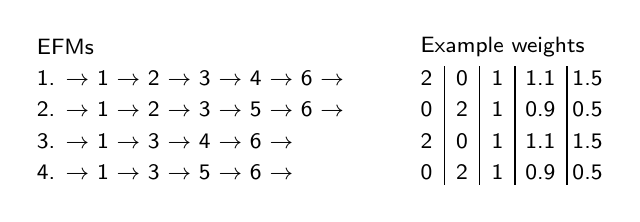
\begin{tikzpicture}[%
    >=latex,
    decoration={%
      markings,
      mark=at position 1.0 with {\arrow{>}}
    },
    every node/.style={%
      font=\sffamily\footnotesize\itshape,
      text=gray,
      text centered,
      align=center
    },
    frame/.style={draw=black,inner sep=2pt}
  ]

  \node[black, font=\sffamily\footnotesize] (t1) {EFMs};
  \node[black, font=\sffamily\footnotesize, below=0.4cm of t1.west, anchor=west]
    (t2)
    {1. $\rightarrow$ 1 $\rightarrow$ 2 $\rightarrow$ 3 $\rightarrow$ 4 $\rightarrow$ 6 $\rightarrow$};
  \node[black, font=\sffamily\footnotesize, below=0.4cm of t2.west, anchor=west]
    (t3)
    {2. $\rightarrow$ 1 $\rightarrow$ 2 $\rightarrow$ 3 $\rightarrow$ 5 $\rightarrow$ 6 $\rightarrow$};
  \node[black, font=\sffamily\footnotesize, below=0.4cm of t3.west, anchor=west]
    (t4)
    {3. $\rightarrow$ 1 $\rightarrow$ 3 $\rightarrow$ 4 $\rightarrow$ 6 $\rightarrow$};
  \node[black, font=\sffamily\footnotesize, below=0.4cm of t4.west, anchor=west]
    (t5)
    {4. $\rightarrow$ 1 $\rightarrow$ 3 $\rightarrow$ 5 $\rightarrow$ 6 $\rightarrow$};

  \node[black, font=\sffamily\footnotesize, right=3.9cm of t1] (u1) {Example weights\textcolor{white}{ss}};
  \node[black, font=\sffamily\footnotesize, below=0.4cm of u1, anchor=south]
    (u2)
    {\textcolor{white}{Example weightsss}};
  \node[black, font=\sffamily\footnotesize, below=0.4cm of u2, anchor=south]
    (u3)
    {\textcolor{white}{Example weightsss}};
  \node[black, font=\sffamily\footnotesize, below=0.4cm of u3, anchor=south]
    (u4)
    {\textcolor{white}{Example weightsss}};
  \node[black, font=\sffamily\footnotesize, below=0.4cm of u1.west, anchor=west]
    (a1)
    {2};
  \node[black, font=\sffamily\footnotesize, below=0.4cm of u1.west, anchor=west,xshift=0.45cm]
    (a2)
    {0};
  \node[black, font=\sffamily\footnotesize, below=0.4cm of u1.west, anchor=west,xshift=0.9cm]
    (a3)
    {1};
  \node[black, font=\sffamily\footnotesize, below=0.4cm of u1.east, anchor=east,xshift=-0.6cm]
    (a4)
    {1.1};
  \node[black, font=\sffamily\footnotesize, below=0.4cm of u1.east, anchor=east,xshift=0cm]
    ()
    {1.5};

  \node[black, font=\sffamily\footnotesize, below=0.4cm of u2.west, anchor=west]
    ()
    {0};
  \node[black, font=\sffamily\footnotesize, below=0.4cm of u2.west, anchor=west,xshift=0.45cm] ()
    {2};
  \node[black, font=\sffamily\footnotesize, below=0.4cm of u2.west, anchor=west,xshift=0.9cm]
    ()
    {1};
  \node[black, font=\sffamily\footnotesize, below=0.4cm of u2.east, anchor=east,xshift=-0.6cm]
    ()
    {0.9};
  \node[black, font=\sffamily\footnotesize, below=0.4cm of u2.east, anchor=east,xshift=0cm]
    ()
    {0.5};
  \node[black, font=\sffamily\footnotesize, below=0.4cm of u3.west, anchor=west]
    ()
    {2};
  \node[black, font=\sffamily\footnotesize, below=0.4cm of u3.west, anchor=west,xshift=0.45cm]
    ()
    {0};
  \node[black, font=\sffamily\footnotesize, below=0.4cm of u3.west, anchor=west,xshift=0.9cm]
    ()
    {1};
  \node[black, font=\sffamily\footnotesize, below=0.4cm of u3.east, anchor=east,xshift=-0.6cm]
    ()
    {1.1};
  \node[black, font=\sffamily\footnotesize, below=0.4cm of u3.east, anchor=east,xshift=0cm]
    ()
    {1.5};

  \node[black, font=\sffamily\footnotesize, below=0.4cm of u4.west, anchor=west]
    (b1)
    {0};
  \node[black, font=\sffamily\footnotesize, below=0.4cm of u4.west, anchor=west,xshift=0.45cm]
    (b2)
    {2};
  \node[black, font=\sffamily\footnotesize, below=0.4cm of u4.west, anchor=west,xshift=0.9cm]
    (b3)
    {1};
  \node[black, font=\sffamily\footnotesize, below=0.4cm of u4.east, anchor=east,xshift=-0.6cm]
    (b4)
    {0.9};
  \node[black, font=\sffamily\footnotesize, below=0.4cm of u4.east, anchor=east,xshift=0cm]
    ()
    {0.5};

  % Vertical bars
  \node[black, right=0.1cm of a1, xshift=-2.0mm,yshift=+1.5mm] (l1) {};
  \node[black, right=0.1cm of b1, xshift=-2.0mm,yshift=-1.5mm] (m1) {};
  \draw[black] (l1.center) to (m1.center);
  \node[black, right=0.1cm of a2, xshift=-2.0mm,yshift=+1.5mm] (l2) {};
  \node[black, right=0.1cm of b2, xshift=-2.0mm,yshift=-1.5mm] (m2) {};
  \draw[black] (l2.center) to (m2.center);
  \node[black, right=0.1cm of a3, xshift=-2.0mm,yshift=+1.5mm] (l3) {};
  \node[black, right=0.1cm of b3, xshift=-2.0mm,yshift=-1.5mm] (m3) {};
  \draw[black] (l3.center) to (m3.center);
  \node[black, right=0.1cm of a4, xshift=-2.0mm,yshift=+1.5mm] (l4) {};
  \node[black, right=0.1cm of b4, xshift=-2.0mm,yshift=-1.5mm] (m4) {};
  \draw[black] (l4.center) to (m4.center);


\end{tikzpicture}

}
    \end{subfigure}\hfill%
    \begin{subfigure}[t]{0.5\textwidth}
      \caption{}
      \centering
      \sffamily
      \vspace*{-1.0em}
      \scalebox{0.75}{\begin{tikzpicture}[%
  cartoon/.style={%
    {Square[slant=-0.5,length=\the\pgflinewidth]}-{Stealth},
    line width=1.5pt
  },
  every node/.style={%
    %font=\sffamily\footnotesize\itshape,
    font=\sffamily\footnotesize,
    text=black,
    text centered,
    align=center
  },
  frame/.style={draw=black,inner sep=2pt}
]
  % Nodes
  \node[lnodeB] (A1) {L-Glutamate\\(1)};
  \node[below=1.0cm of A1] (P1) {};
  \node[lnodeB,right=1.5cm of P1,anchor=center] (A2) {L-Glutamyl 5-phosphate\\(2)};
  \node[lnodeB,below=1.0cm of P1] (A3) {L-Glutamate 5-semialdehyde\\(3)};
  \node[below=1.0cm of A3] (P2) {};
  \node[lnodeB,left=1.5cm of P2,anchor=center] (A4) {(S)-1-Pyrroline-5-carboxylate\\(4)};
  \node[lnodeB,right=1.5cm of P2,anchor=center] (A5) {L-Ornithine\\(5)};
  \node[lnodeB,below=1.0cm of P2] (A6) {L-Proline\\(6)};
  \node[above=0.5cm of A1] (Y1) {};
  \node[below=0.5cm of A6] (Y2) {};

  \node[lnodeB] at (A1) (B1) {5,6,7,8-Tetrahydrofolate (THF)\\(1)};
  \node[lnodeB] at (A6) (B4) {5-Formimino-THF\\(4)};
  \node (P1) at ($(B1)!0.333!(B4)$) {};
  \node (P2) at ($(B1)!0.667!(B4)$) {};
  \node[lnodeB] at (P1) (B2) {10-Formyl-THF\\(2)};
  \node[lnodeB] at (P2) (B3) {5,10-Methenyl-THF\\(3)};
  \node[above=0.5cm of B1] (Y1) {};
  \node[below=0.5cm of B4] (Y2) {};
  \node[left=0.75cm of A3] (P3) {3 \quad 2};

  % Intra-node edges
  \draw[postaction={decorate},cartoon] (B1.center) to [bend right=40] node [below right=0.1pt,yshift=-0pt] {3} (B2);
  \draw[postaction={decorate},cartoon] (B2.center) to [bend right=40] node [below left=0.1pt,yshift=+12.4pt] {2} (B1);
  \draw[postaction={decorate},cartoon] (B2.center) to [bend right=40] node [below right=0.1pt,yshift=-0pt] {3} (B3);
  \draw[postaction={decorate},cartoon] (B3.center) to [bend right=40] node [below left=0.1pt,yshift=+12pt] {2} (B2);
  \draw[postaction={decorate},cartoon] (B3.center) to [bend right=40] node [below right=0.1pt,yshift=-0pt] {2} (B4);
  \draw[postaction={decorate},cartoon] (B4.center) to [bend right=40] node [below left=0.1pt,yshift=+12.4pt] {3} (B3);
  \draw[cartoon,rounded corners=15pt] ([xshift=-0.4cm]B3.center) to [bend left=40] node [left=0.1pt] {2} ([xshift=-0.4cm]B1.south);

  \draw[-,line width=1.5pt,rounded corners=15pt] ([yshift=+0.1cm]B4.center) -| ([xshift=+0.1cm]P3.center);
  \draw[cartoon,rounded corners=15pt] ([xshift=+0.1cm,yshift=-3pt]P3.center) |- ([yshift=-0.1cm]B1.west);
  \draw[-,line width=1.5pt,rounded corners=15pt] ([yshift=+0.1cm]B1.center) -| ([xshift=-0.1cm,yshift=-3pt]P3.center);
  \draw[cartoon,rounded corners=15pt] ([xshift=-0.1cm]P3.center) |- ([yshift=-0.1cm]B4.west);

  % Repeat nodes
  \node[lnodeB] at (B1) (B1) {5,6,7,8-Tetrahydrofolate (THF)\\(1)};
  \node[lnode2] at (B1) (B1) {5,6,7,8-Tetrahydrofolate (THF)\\(1)};
  \node[lnodeB] at (B4) (B4) {5-Formimino-THF\\(4)};
  \node[lnode2] at (B4) (B4) {5-Formimino-THF\\(4)};
  \node[lnodeB] at (B2) (B2) {10-Formyl-THF\\(2)};
  \node[lnode2] at (B2) (B2) {10-Formyl-THF\\(2)};
  \node[lnodeB] at (B3) (B3) {5,10-Methenyl-THF\\(3)};
  \node[lnode2] at (B3) (B3) {5,10-Methenyl-THF\\(3)};

  % Boundary edges
  %\draw[cartoon,tbGray] (Y1.center) to node [left,yshift=5pt] {} (A1.north);
  %\draw[cartoon,tbGray] (A7.center) to node [left] {} (Y2.center);

  \node[rectangle,width=0.1cm,fill=white,above=0.60cm of A1] (Z) {};

\end{tikzpicture}


}\\ % https://www.genome.jp/pathway/map00670
      \vspace*{-0.5em}
      \scalebox{0.75}{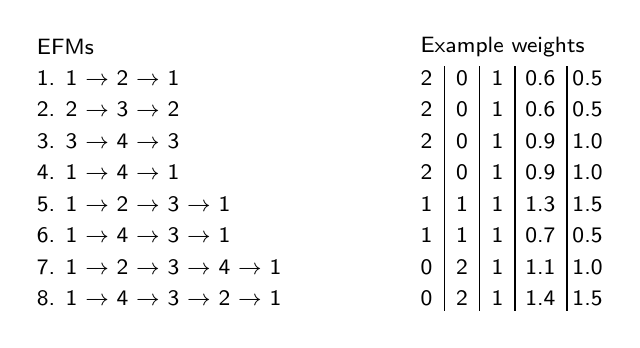
\begin{tikzpicture}[%
    >=latex,
    decoration={%
      markings,
      mark=at position 1.0 with {\arrow{>}}
    },
    every node/.style={%
      font=\sffamily\footnotesize\itshape,
      text=gray,
      text centered,
      align=center
    },
    frame/.style={draw=black,inner sep=2pt}
  ]

  \node[black, font=\sffamily\footnotesize] (t1) {EFMs};
  \node[black, font=\sffamily\footnotesize, below=0.4cm of t1.west, anchor=west]
    (t2)
    {1. 1 $\rightarrow$ 2 $\rightarrow$ 1};
  \node[black, font=\sffamily\footnotesize, below=0.4cm of t2.west, anchor=west]
    (t3)
    {2. 2 $\rightarrow$ 3 $\rightarrow$ 2};
  \node[black, font=\sffamily\footnotesize, below=0.4cm of t3.west, anchor=west]
    (t4)
    {3. 3 $\rightarrow$ 4 $\rightarrow$ 3};
  \node[black, font=\sffamily\footnotesize, below=0.4cm of t4.west, anchor=west]
    (t5)
    {4. 1 $\rightarrow$ 4 $\rightarrow$ 1};
  \node[black, font=\sffamily\footnotesize, below=0.4cm of t5.west, anchor=west]
    (t6)
    {5. 1 $\rightarrow$ 2 $\rightarrow$ 3 $\rightarrow$ 1};
  \node[black, font=\sffamily\footnotesize, below=0.4cm of t6.west, anchor=west]
    (t7)
    {6. 1 $\rightarrow$ 4 $\rightarrow$ 3 $\rightarrow$ 1};
  \node[black, font=\sffamily\footnotesize, below=0.4cm of t7.west, anchor=west]
    (t8)
    {7. 1 $\rightarrow$ 2 $\rightarrow$ 3 $\rightarrow$ 4 $\rightarrow$ 1};
  \node[black, font=\sffamily\footnotesize, below=0.4cm of t8.west, anchor=west]
    (t9)
    {8. 1 $\rightarrow$ 4 $\rightarrow$ 3 $\rightarrow$ 2 $\rightarrow$ 1};

  \node[black, font=\sffamily\footnotesize, right=3.9cm of t1] (u1) {Example weights\textcolor{white}{ss}};
  \node[black, font=\sffamily\footnotesize, below=0.4cm of u1, anchor=south]
    (u2)
    {\textcolor{white}{Example weightsss}};
  \node[black, font=\sffamily\footnotesize, below=0.4cm of u2, anchor=south]
    (u3)
    {\textcolor{white}{Example weightsss}};
  \node[black, font=\sffamily\footnotesize, below=0.4cm of u3, anchor=south]
    (u4)
    {\textcolor{white}{Example weightsss}};
  \node[black, font=\sffamily\footnotesize, below=0.4cm of u4, anchor=south]
    (u5)
    {\textcolor{white}{Example weightsss}};
  \node[black, font=\sffamily\footnotesize, below=0.4cm of u5, anchor=south]
    (u6)
    {\textcolor{white}{Example weightsss}};
  \node[black, font=\sffamily\footnotesize, below=0.4cm of u6, anchor=south]
    (u7)
    {\textcolor{white}{Example weightsss}};
  \node[black, font=\sffamily\footnotesize, below=0.4cm of u7, anchor=south]
    (u8)
    {\textcolor{white}{Example weightsss}};

  \node[black, font=\sffamily\footnotesize, below=0.4cm of u1.west, anchor=west]
    (a1)
    {2};
  \node[black, font=\sffamily\footnotesize, below=0.4cm of u1.west, anchor=west,xshift=0.45cm]
    (a2)
    {0};
  \node[black, font=\sffamily\footnotesize, below=0.4cm of u1.west, anchor=west,xshift=0.9cm]
    (a3)
    {1};
  \node[black, font=\sffamily\footnotesize, below=0.4cm of u1.east, anchor=east,xshift=-0.6cm]
    (a4)
    {0.6};
  \node[black, font=\sffamily\footnotesize, below=0.4cm of u1.east, anchor=east,xshift=0cm]
    ()
    {0.5};

  \node[black, font=\sffamily\footnotesize, below=0.4cm of u2.west, anchor=west]
    ()
    {2};
  \node[black, font=\sffamily\footnotesize, below=0.4cm of u2.west, anchor=west,xshift=0.45cm]
    ()
    {0};
  \node[black, font=\sffamily\footnotesize, below=0.4cm of u2.west, anchor=west,xshift=0.9cm]
    ()
    {1};
  \node[black, font=\sffamily\footnotesize, below=0.4cm of u2.east, anchor=east,xshift=-0.6cm]
    ()
    {0.6};
  \node[black, font=\sffamily\footnotesize, below=0.4cm of u2.east, anchor=east,xshift=0cm]
    ()
    {0.5};

  \node[black, font=\sffamily\footnotesize, below=0.4cm of u3.west, anchor=west]
    ()
    {2};
  \node[black, font=\sffamily\footnotesize, below=0.4cm of u3.west, anchor=west,xshift=0.45cm]
    ()
    {0};
  \node[black, font=\sffamily\footnotesize, below=0.4cm of u3.west, anchor=west,xshift=0.9cm]
    ()
    {1};
  \node[black, font=\sffamily\footnotesize, below=0.4cm of u3.east, anchor=east,xshift=-0.6cm]
    ()
    {0.9};
  \node[black, font=\sffamily\footnotesize, below=0.4cm of u3.east, anchor=east,xshift=0cm]
    ()
    {1.0};

  \node[black, font=\sffamily\footnotesize, below=0.4cm of u4.west, anchor=west]
    (b1)
    {2};
  \node[black, font=\sffamily\footnotesize, below=0.4cm of u4.west, anchor=west,xshift=0.45cm]
    (b2)
    {0};
  \node[black, font=\sffamily\footnotesize, below=0.4cm of u4.west, anchor=west,xshift=0.9cm]
    (b3)
    {1};
  \node[black, font=\sffamily\footnotesize, below=0.4cm of u4.east, anchor=east,xshift=-0.6cm]
    (b4)
    {0.9};
  \node[black, font=\sffamily\footnotesize, below=0.4cm of u4.east, anchor=east,xshift=0cm]
    ()
    {1.0};

  \node[black, font=\sffamily\footnotesize, below=0.4cm of u5.west, anchor=west]
    (b1)
    {1};
  \node[black, font=\sffamily\footnotesize, below=0.4cm of u5.west, anchor=west,xshift=0.45cm]
    (b2)
    {1};
  \node[black, font=\sffamily\footnotesize, below=0.4cm of u5.west, anchor=west,xshift=0.9cm]
    (b3)
    {1};
  \node[black, font=\sffamily\footnotesize, below=0.4cm of u5.east, anchor=east,xshift=-0.6cm]
    (b4)
    {1.3};
  \node[black, font=\sffamily\footnotesize, below=0.4cm of u5.east, anchor=east,xshift=0cm]
    ()
    {1.5};

  \node[black, font=\sffamily\footnotesize, below=0.4cm of u6.west, anchor=west]
    (b1)
    {1};
  \node[black, font=\sffamily\footnotesize, below=0.4cm of u6.west, anchor=west,xshift=0.45cm]
    (b2)
    {1};
  \node[black, font=\sffamily\footnotesize, below=0.4cm of u6.west, anchor=west,xshift=0.9cm]
    (b3)
    {1};
  \node[black, font=\sffamily\footnotesize, below=0.4cm of u6.east, anchor=east,xshift=-0.6cm]
    (b4)
    {0.7};
  \node[black, font=\sffamily\footnotesize, below=0.4cm of u6.east, anchor=east,xshift=0cm]
    ()
    {0.5};

  \node[black, font=\sffamily\footnotesize, below=0.4cm of u7.west, anchor=west]
    (b1)
    {0};
  \node[black, font=\sffamily\footnotesize, below=0.4cm of u7.west, anchor=west,xshift=0.45cm]
    (b2)
    {2};
  \node[black, font=\sffamily\footnotesize, below=0.4cm of u7.west, anchor=west,xshift=0.9cm]
    (b3)
    {1};
  \node[black, font=\sffamily\footnotesize, below=0.4cm of u7.east, anchor=east,xshift=-0.6cm]
    (b4)
    {1.1};
  \node[black, font=\sffamily\footnotesize, below=0.4cm of u7.east, anchor=east,xshift=0cm]
    ()
    {1.0};

  \node[black, font=\sffamily\footnotesize, below=0.4cm of u8.west, anchor=west]
    (b1)
    {0};
  \node[black, font=\sffamily\footnotesize, below=0.4cm of u8.west, anchor=west,xshift=0.45cm]
    (b2)
    {2};
  \node[black, font=\sffamily\footnotesize, below=0.4cm of u8.west, anchor=west,xshift=0.9cm]
    (b3)
    {1};
  \node[black, font=\sffamily\footnotesize, below=0.4cm of u8.east, anchor=east,xshift=-0.6cm]
    (b4)
    {1.4};
  \node[black, font=\sffamily\footnotesize, below=0.4cm of u8.east, anchor=east,xshift=0cm]
    ()
    {1.5};

  % Vertical bars
  \node[black, right=0.1cm of a1, xshift=-2.0mm,yshift=+1.5mm] (l1) {};
  \node[black, right=0.1cm of b1, xshift=-2.0mm,yshift=-1.5mm] (m1) {};
  \draw[black] (l1.center) to (m1.center);
  \node[black, right=0.1cm of a2, xshift=-2.0mm,yshift=+1.5mm] (l2) {};
  \node[black, right=0.1cm of b2, xshift=-2.0mm,yshift=-1.5mm] (m2) {};
  \draw[black] (l2.center) to (m2.center);
  \node[black, right=0.1cm of a3, xshift=-2.0mm,yshift=+1.5mm] (l3) {};
  \node[black, right=0.1cm of b3, xshift=-2.0mm,yshift=-1.5mm] (m3) {};
  \draw[black] (l3.center) to (m3.center);
  \node[black, right=0.1cm of a4, xshift=-2.0mm,yshift=+1.5mm] (l4) {};
  \node[black, right=0.1cm of b4, xshift=-2.0mm,yshift=-1.5mm] (m4) {};
  \draw[black] (l4.center) to (m4.center);


\end{tikzpicture}

}
    \end{subfigure}
  \end{figure}
\end{document}

